\documentclass{article}

    \usepackage[utf8]{inputenc}
    \usepackage[T1]{fontenc}
    \usepackage{float}
    \usepackage[french]{babel}
    \usepackage[margin=.8in]{geometry}
    \usepackage{amssymb}
    \usepackage{amsmath}  
    \usepackage{mathtools}
    \usepackage{listings}
    \usepackage{graphicx}
    \usepackage[hidelinks]{hyperref}
    \usepackage{calrsfs}
    \usepackage{bookmark}
    \usepackage{tikz,tkz-tab}
    \DeclarePairedDelimiter\abs{\lvert}{\rvert}%
    \DeclarePairedDelimiter\bigabs{\Big\lvert}{\Big\rvert}%
    \DeclarePairedDelimiter{\ceil}{\lceil}{\rceil}
    \newcommand{\Mod}[1]{\ (\mathrm{mod}\ #1)}
    
\begin{document}

\title{Projet 3 - MATH04 \\ Les séries de Fourier}
\author{Nathan Soufflet}

\maketitle
\pagenumbering{gobble}
\newpage

\section{Etude d'une série de fonctions}

Soit $f_n(x) = \frac{2 (-1)^{n + 1}\sin(nx)}{n}$

\begin{figure}[ht!]
    \centering
    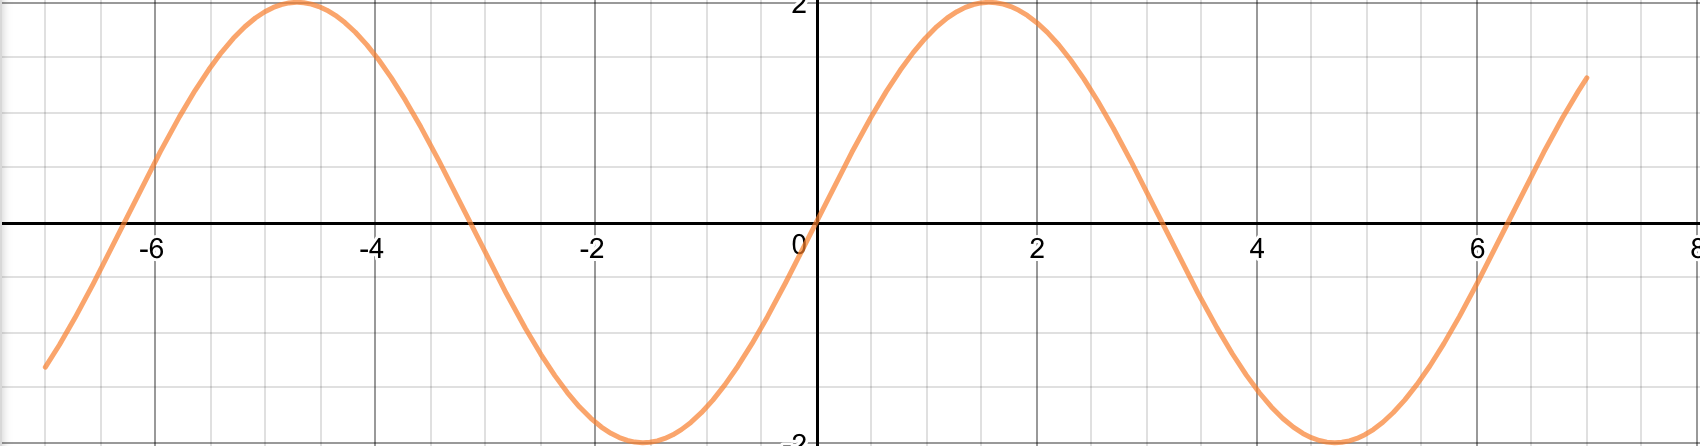
\includegraphics[width=\textwidth]{figures/f_n_1.png}
    \caption{$f_{1}(x)$ sur $[-7, 7]$}
\end{figure}

\begin{figure}[ht!]
    \centering
    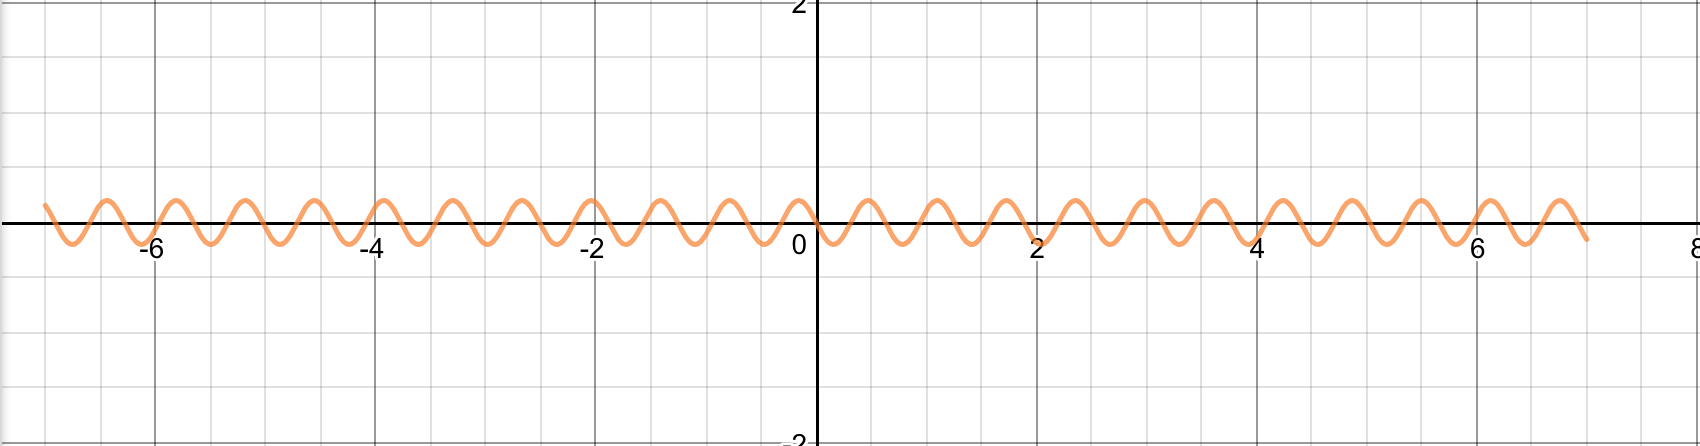
\includegraphics[width=\textwidth]{figures/f_n_10.png}
    \caption{$f_{10}(x)$ sur $[-7, 7]$}
\end{figure}

\begin{figure}[ht!]
    \centering
    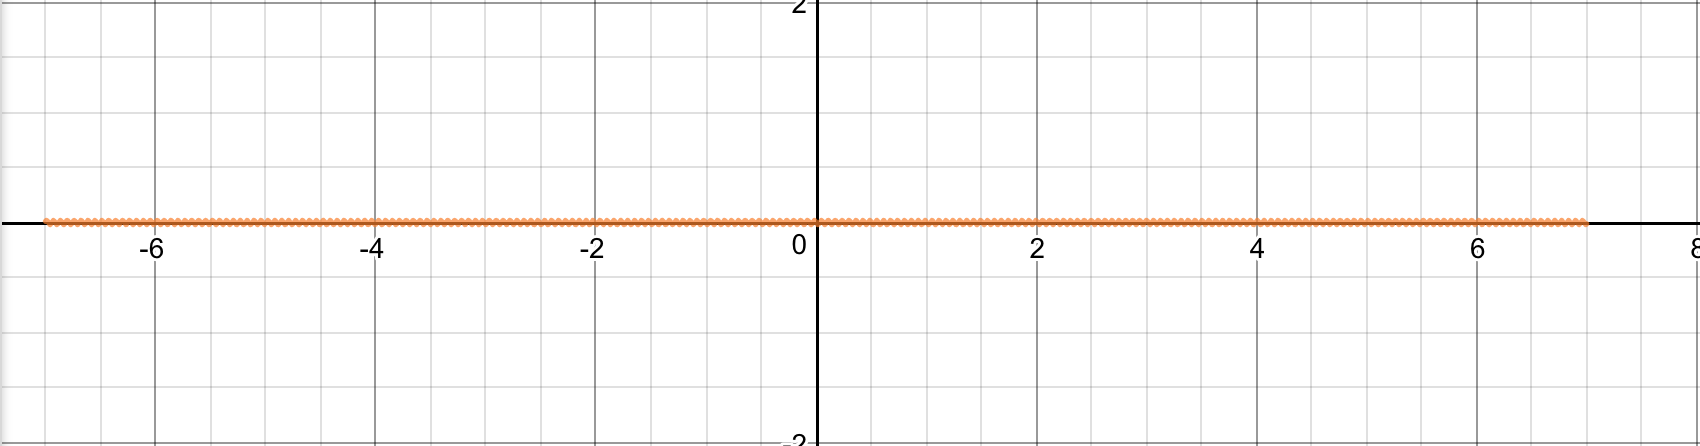
\includegraphics[width=\textwidth]{figures/f_n_100.png}
    \caption{$f_{100}(x)$ sur $[-7, 7]$}
\end{figure}

L'observation numérique du comportement de $f_n(x)$ quand $n$ augmente semble vérifier l'hypothèse que
la suite $(f_n)$ converge simplement vers la fonction nulle.

\newpage

\begin{figure}[ht!]
    \centering
    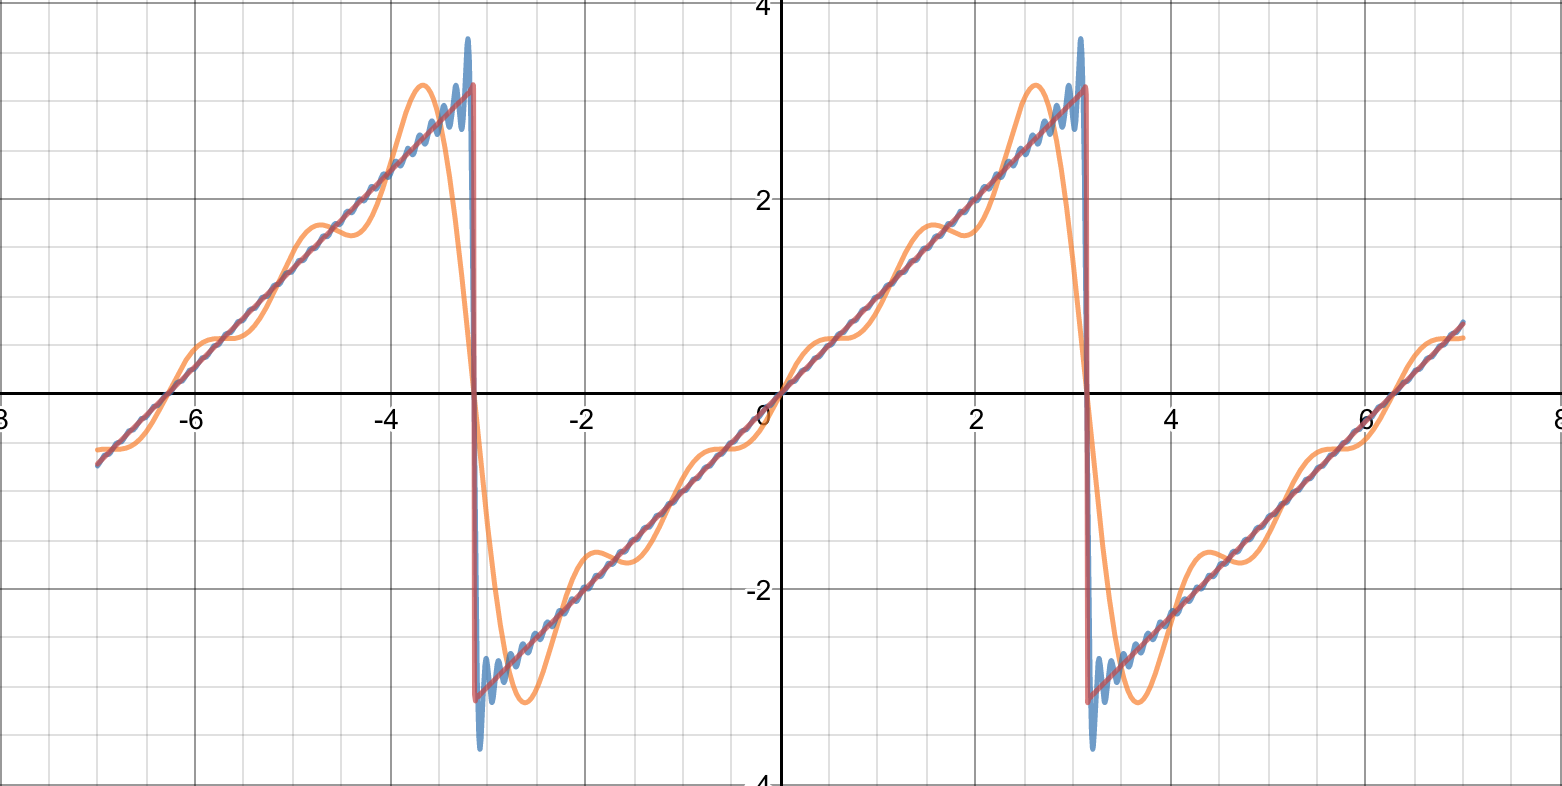
\includegraphics[width=0.8\textwidth]{figures/S_n.png}
    \caption{Suite des sommes partielles de la série de terme général $f_n$ pour $n = 5, 50$ et $5000$}
\end{figure}

Ce graphique permet de conjecturer que la suite de terme général $f_n$ converge vers un signal en dents de scie
$2\pi$-{périodique} d'amplitude $\pi$ : $f(x) = x - \pi \Mod{2\pi} - \pi$

\begin{figure}[ht!]
    \centering
    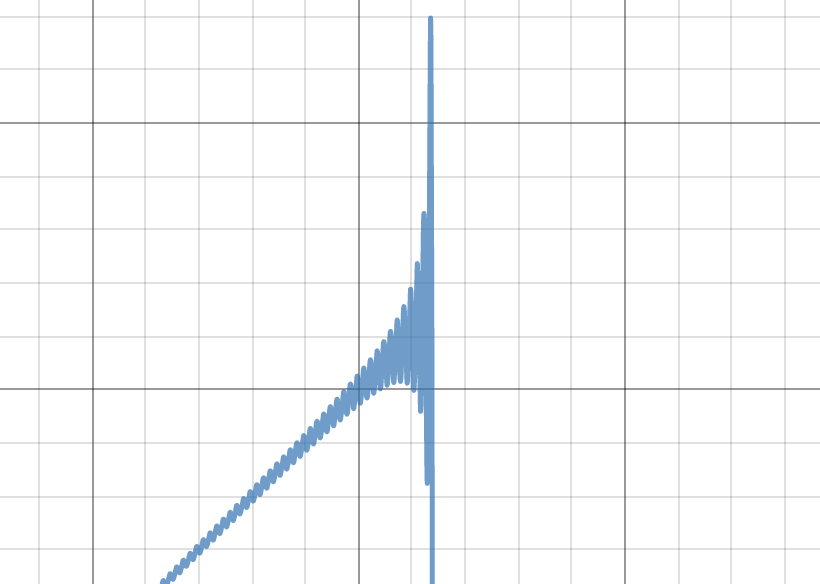
\includegraphics[height=0.35\textwidth]{figures/gibbs.png}
    \caption{Phénomène de Gibbs près de $x = 3.14$, pour $n = 500$}
\end{figure}

Dans un voisinage de $x = \pi$, on observe une amplification de la discontinuité de la fonction somme en ce point
(Phénomène de Gibbs). \\

En $x = \frac{\pi}{2}$, on a $\sin(nx) = \sin(\frac{n\pi}{2})$

\begin{equation*}
    \sin(\frac{n\pi}{2}) = \left \{
    \begin{aligned}
      &0 && \text{si}\ n \text{ pair} \\
      &(-1)^{\frac{n - 1}{2}} && \text{sinon}
    \end{aligned} \right.
\end{equation*} 

ainsi, seuls les termes impairs sont non-nuls, par changement de variable on obtient :

$$\sum_{n = 1}^{\infty}{\frac{2 (-1)^{n + 1}\sin(\frac{n\pi}{2})}{n}} = 2 \sum_{p = 0}^{\infty}{\frac{(-1)^p}{2p+1}}
= f(\frac{\pi}{2})$$

or $f(\frac{\pi}{2}) = \frac{\pi}{2}$ d'où :

$$\sum_{p = 0}^{\infty}{\frac{(-1)^p}{2p+1}} = \frac{\pi}{4}$$

\section{Convergence}

\subsection{Lemme de Riemann-Lebesgue}

Par intégration par partie, on a : 

$$\int_{a}^{b}{f(t) \sin(\lambda t) dt} = \frac{1}{\lambda}\Big[ \cos(\lambda a) f(a) - \cos(\lambda b)
f(b) + \int_{a}^{b}{f'(t) \cos(\lambda t)} \Big]$$

Par continuité de $f$ et $f'$ sur $[a, b]$, $f$ et $f'$ sont bornées et donc majorées sur $[a, b]$
on en déduit l'existence d'un majorant $M \in \mathbb{R}^{+}$ de 
$|\cos(\lambda a) f(a) - \cos(\lambda b) f(b) + \int_{a}^{b}{f'(t) \cos(\lambda t)}|$ d'où :

$$\lim_{\lambda \to \infty} \int_{a}^{b}{|f(t) \sin(\lambda t)| dt} \leq 
\lim_{\lambda \to \infty} \frac{M}{\lambda} = 0$$

Par conséquent : 

$$\lim_{\lambda \to \infty} \int_{a}^{b}{f(t) \sin(\lambda t) dt} = 0$$

\subsection{Noyau de Dirichlet}

    Soit $D(\theta) = \frac{1}{2} + \sum_{k = 1}^{n} \cos(n \theta)$ \\

    En multipliant des deux côtés par $2\sin(\frac{\theta}{2})$, et en utilisant l'identité du produit 
    de deux cosinus, on a :

    $$2\sin(\frac{\theta}{2}) D(\theta) = \sin(\frac{\theta}{2}) + \sum_{k = 1}^{n} 
    \sin(\theta (k + \frac{1}{2})) - \sin(\theta (k - \frac{1}{2}))$$

    Qui est une somme telescopique, que l'on peut simplifier comme suit :

    $$2\sin(\frac{\theta}{2}) D(\theta) = \sin(\frac{\theta}{2}) + \sin(\theta (n + \frac{1}{2})) - \sin(\frac{\theta}{2})$$

    On en déduit :

    $$D(\theta) = \frac{\sin(\theta (n + \frac{1}{2}))}{2\sin(\frac{\theta}{2})}$$

\subsection{Theoreme de Dirichlet}

\subsubsection{}
$$S_{N}(x) = \frac{a_0}{2} + \sum_{n = 1}^{N} a_n \cos(nx) + b_n \sin(nx)$$

En substituant $a_n$ et $b_n$ : 

$$S_{N}(x) = \frac{a_0}{2} + \sum_{n = 1}^{N} \frac{1}{\pi}\Big[
    \int_{0}^{2\pi} f(t) \cos(nt) \cos(nx) dt + \int_{0}^{2\pi} f(t) \sin(nt) \sin(nx) dt
\Big]$$

Par interversion de la somme et de l'intégrale et en utilisant les identités du produit de deux cosinus et sinus :

$$S_{N}(x) = a_0 + \frac{1}{\pi} \int_{0}^{2\pi} \sum_{n = 1}^{N} f(t) \cos(n (t + x)) dt$$

or $a_0 = \frac{1}{\pi} \int_{0}^{2\pi} f(t) dt$ d'où :

$$S_{N}(x) = \frac{1}{\pi} \int_{0}^{2\pi} \sum_{n = 1}^{N} \Big[\frac{1}{2} + \cos(n (t + x))\Big] f(t) dt$$

\subsubsection{}
On a :

$$D(\theta) = \frac{\sin(\theta (N + \frac{1}{2}))}{2\sin(\frac{\theta}{2})}
= \frac{\sin(\frac{\theta}{2} (2N + 1))}{2\sin(\frac{\theta}{2})}$$

d'où, avec le changement de variable $\theta = t - x$ : 

$$S_{N}(x) = \frac{1}{2\pi} \int_{0}^{2\pi} f(\theta + x) \frac{\sin(\frac{\theta}{2} (2N + 1))}{\sin(\frac{\theta}{2})}$$

\subsubsection{}
En découpant l'intégrale en deux :

$$I = \int_{0}^{\pi} \Big[f(x + t) + f(x - t)\Big] 2D(t) dt = \int_{0}^{\pi} f(x + t) 2D(t) dt
+ \int_{0}^{\pi} f(x - t) 2D(t) dt$$

Par périodicité de $f(x)$ :

$$I = \int_{0}^{\pi} f(x + t) 2D(t) dt + \int_{\pi}^{2\pi} f(x + t) 2D(t) dt =
\int_{0}^{2\pi} f(x + t) 2D(t) dt = 2\pi S_N(x)$$ 

Soit la fonction $f(x) = \frac{1}{2}$, on déduit du résultat précédent que :

$$\frac{1}{2} = \frac{1}{2\pi} \int_{0}^{\pi} 2 D(t) dt$$

d'où $\frac{1}{\pi} \int_{0}^{\pi} 2 D(t) dt = 1$

\subsubsection{}

Soit $\epsilon_N(x) = S_N(x) - \frac{1}{2}(f(x_{+}) + f(x_{-}))$

En multipliant la dernière égalité par la constante $\frac{1}{2}\Big[f(x_{+}) + f(x_{-})\Big]$ :

$$\frac{1}{2}\Big[f(x_{+}) + f(x_{-})\Big] =
\frac{1}{2\pi} \int_{0}^{\pi} \frac{f(x + t) + f(x - t)}{\sin(\frac{t}{2})} \sin((2N + 1)\frac{\theta}{2}) dt$$


D'où :

$$\epsilon_N(x) = \frac{1}{2\pi} \int_{0}^{\pi} 
\frac{f(x + t) - f(x - t) - f(x_{+}) - f(x_{-})}{\sin(\frac{t}{2})} \sin((2N + 1)\frac{\theta}{2}) dt$$

Finalement :

$$\epsilon_N(x) = \frac{1}{2\pi} \int_{0}^{\pi} g_{x}(t) \sin((2N + 1)\frac{\theta}{2}) dt$$

Par continuité de $g$, on peut alors appliquer le lemme de Riemann-Lebesgue :

$$\lim_{N \to \infty} \epsilon_N(x) = 0 \Rightarrow \lim_{N \to \infty} S_N(x) = \frac{1}{2}\Big[f(x_{+}) + f(x_{-})\Big]$$

Ce qui démontre le théorème de Dirichlet.

\section{Application du theoreme de Dirichlet}

\subsection{Retour au premier exemple}

\subsubsection{}

Soit la fonction $2\pi$-périodique $f$ telle que $f(x) = x, \forall x \in ]-\pi, \pi[$ et $f(\pi) = 0$

$f(x)$ etant impaire, seuls les coefficients $b_n$ sont non-nuls :

$$b_n = \frac{1}{\pi} \int_{0}^{2\pi}t \sin(n t) dt$$

En intégrant par partie, on obtient :

$$b_n = \frac{-2 \cos(2 \pi n)}{n} = \frac{2(-1)^{n+1}}{n}$$

\subsubsection{}

En appliquant le lemme de Riemann-Lebesgue, on confirme que $(f_n)$ converge simplement vers la fonction nulle :

$$\lim_{n \to \infty} \frac{2(-1)^{n+1}}{n} \sin(n x) = 0$$

D'après le théorème de Dirichlet (sur $]-\pi, \pi[$)

$$\sum_{n = 1}^{\infty} \frac{2(-1)^{n+1} \sin(n x)}{n} = f(x)$$

Donc la série étudiée en première partie converge bien vers $f(x)$.

Le résultat $\sum_{p = 0}^{\infty} \frac{(-1)^{p}}{2p + 1} = \frac{\pi}{4}$ est donc valide.

\subsection{Un autre exemple}

\subsubsection{}

Soit la fonction $2\pi$-périodique $f$ telle que $f(x) = |x|$

$f(x)$ etant paire, seuls les coefficients $a_n$ sont non-nuls :

$$a_n = \frac{1}{\pi} \int_{0}^{2\pi}t \cos(n t) dt = \frac{2}{\pi} \int_{0}^{\pi}t \cos(n t) dt$$

En intégrant par partie, on obtient ($\forall n \in \mathbb{N}^*$) : 

\begin{equation*}
    a_n = \left \{
    \begin{aligned}
      &0 && \text{si}\ n \text{ pair} \\
      &-\frac{4}{\pi n^2} && \text{sinon}
    \end{aligned} \right.
\end{equation*} 

et $a_0 = \pi$, d'où :

$$f(x) = \frac{\pi}{2} - \sum_{n = 0}^{\infty} \frac{4 \cos((2n + 1) x)}{\pi(2n + 1)^2}$$

\subsubsection{}

\begin{figure}[ht!]
    \centering
    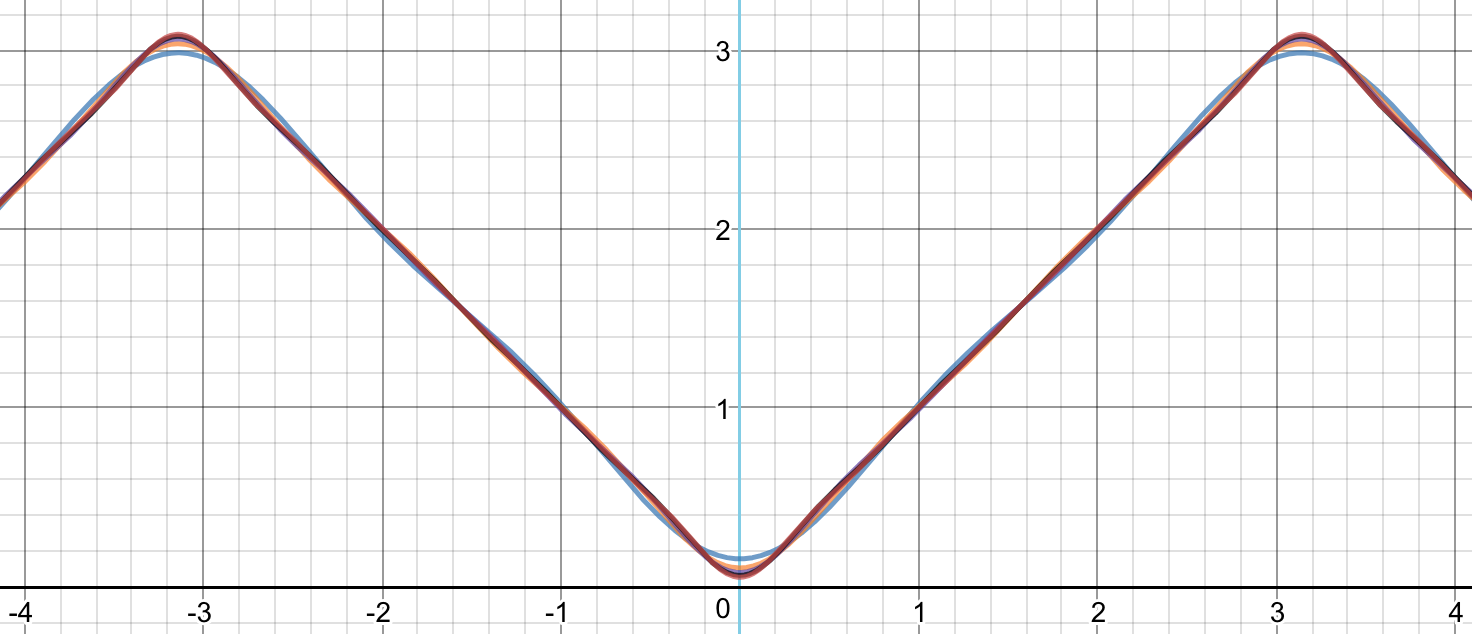
\includegraphics[width=0.7\textwidth]{figures/abs.png}
    \caption{$5$ premières sommes partielles de la série de Fourier de $f(x)$}
\end{figure}

On observe que le phénomène de Gibbs n'est pas apparent pour $f(x) = |x|$ (voir Fig. 6)

\subsubsection{}

$\forall n \in \mathbb{N}, \cos(n \times 0) = 1$ d'où :

$$T = \sum_{p = 0}^{\infty} \frac{1}{(2p + 1)^2} = \frac{\pi}{4} (\frac{\pi}{2} - f(0)) = \frac{\pi^2}{8}$$


\subsubsection{}

Par décalage d'indice :

$$S - T = \sum_{n = 1}^{\infty} \frac{1}{n^2} - 
\sum_{n = 1}^{\infty} \frac{1}{(2n - 1)^2} = \sum_{n = 1}^{\infty} \frac{1}{(2n)^2} = \frac{S}{4}$$

d'où :

$$S = \frac{4}{3} T = \frac{\pi^2}{6}$$

\section{Harmoniques d'un signal}

\subsection{}

\begin{figure}[ht!]
    \centering
    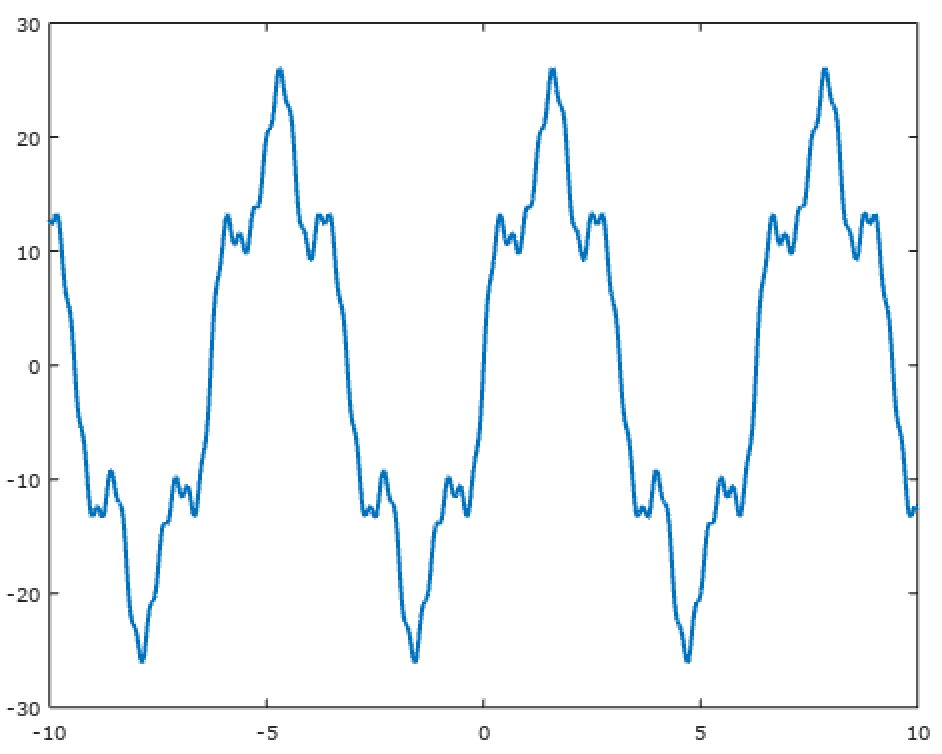
\includegraphics[height=0.35\textwidth]{figures/f_math04.png}
    \caption{$f\_\text{math04}$ sur $[-10, 10]$}
\end{figure}

La fonction $f\_\text{math04}$ semble effectivement $2\pi$-périodique

\subsection{}

Les coefficients de valeur absolue supérieure à $0.05$ sont (pour $n \leq 100$) :

$$\{b_1 \approx 19.99992, b_5 \approx 4.999982, b_8 \approx 0.9993442, b_{21} \approx 0.9956820\}$$

\begin{figure}[ht!]
    \centering
    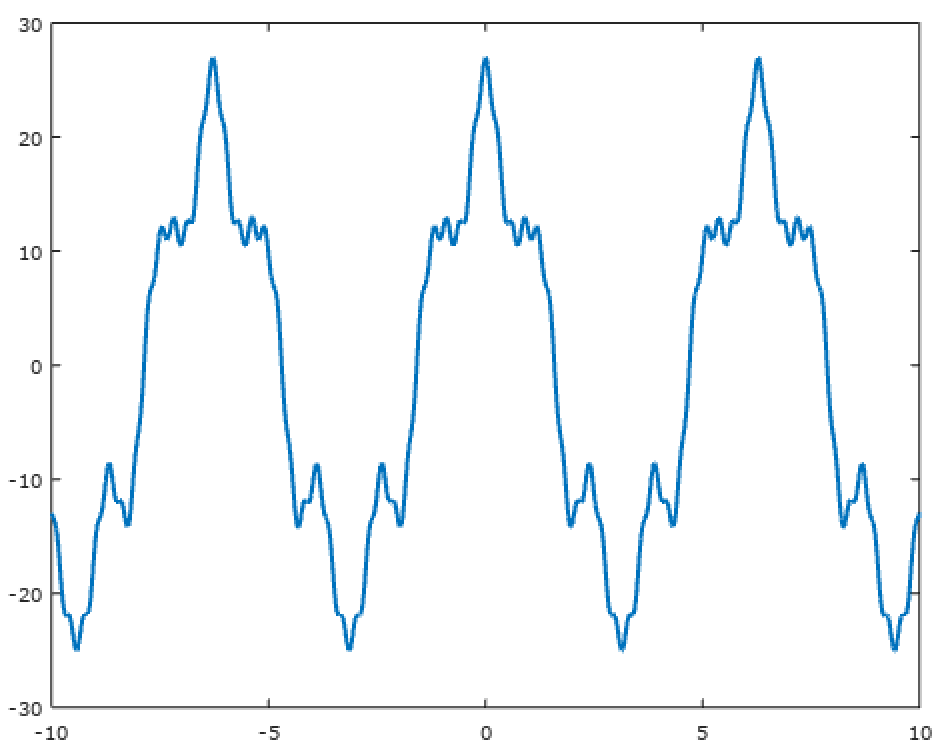
\includegraphics[height=0.3\textwidth]{figures/approx.png}
    \caption{Approximation de $f\_\text{math04}$ sur $[-10, 10]$}
\end{figure}

L'approximation avec les coefficients non-négligeables est cohérente avec la figure 7 (à un décalage près).

\subsection{}

\begin{figure}[ht!]
    \centering
    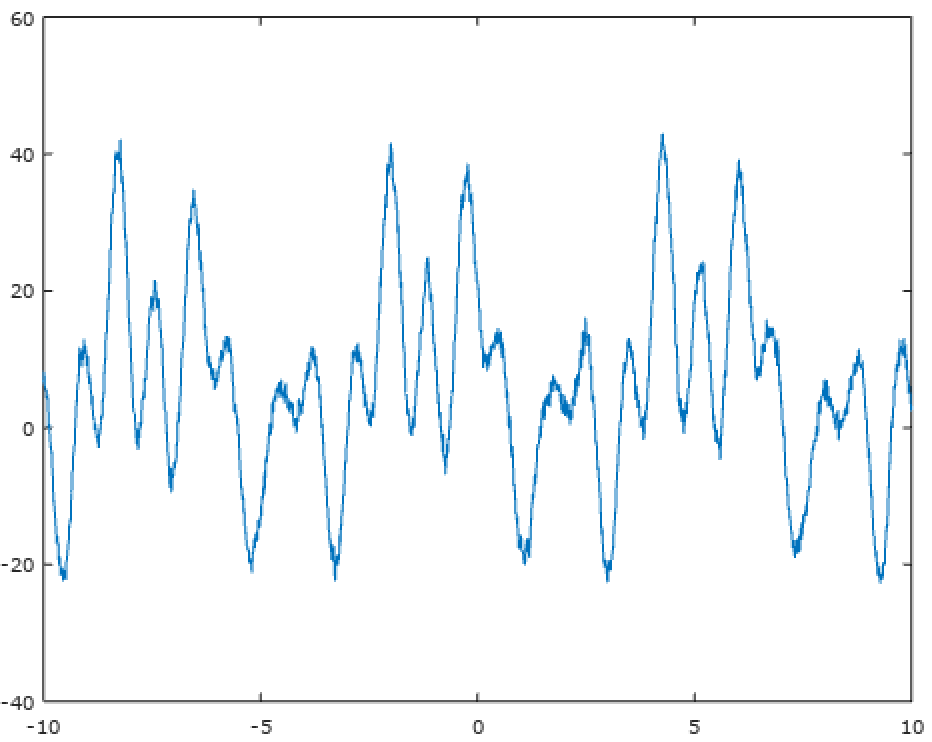
\includegraphics[height=0.3\textwidth]{figures/g_math04.png}
    \caption{$g\_\text{math04}$ sur $[-10, 10]$}
\end{figure}

$g\_\text{math04}(2) = 4.5009$ et $g\_\text{math04}(2 + 2\pi) = 1.6677$, cette fonction n'est donc pas 
$2\pi$-périodique, il faut alors un très grand nombre d'harmoniques pour l'approximer,
en effet, 56 coefficients $a_n$ et 55 $b_n$, pour $n \leq 100$ sont de valeur absolue supérieure à 0.05.
\begin{figure}[ht!]
    \centering
    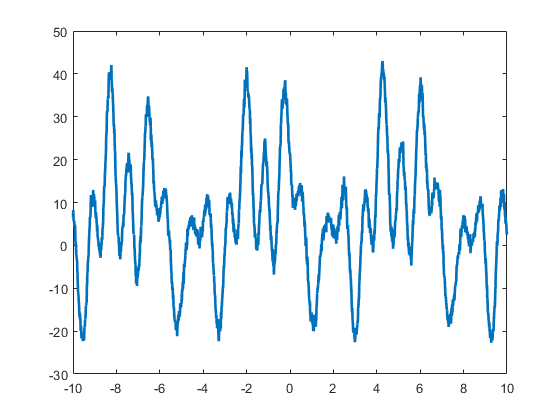
\includegraphics[height=0.3\textwidth]{figures/approx_g.png}
    \caption{Approximation de  $g\_\text{math04}$ sur $[-10, 10]$}
\end{figure}

\end{document}